%% Springer Nature sn-jnl article -- LRFM max-k-cut customer segmentation
%% Submit as a single .tex document. Compile with pdflatex + bibtex.
\documentclass[pdflatex,sn-mathphys-num]{sn-jnl}% Math and Physical Sciences Numbered Reference Style

%% Only packages actually used by this article are loaded.
\usepackage{graphicx}%
\usepackage{amsmath,amssymb,amsfonts}%
\usepackage{textcomp}%      % \textsterling
\usepackage{booktabs}%      % \toprule \midrule
\usepackage{algorithm}%     % Algorithm 1 float
\usepackage{algorithmicx}%
\usepackage{algpseudocode}%

\raggedbottom

\begin{document}

\title[LRFM Max-k-cut Customer Segmentation]{An LRFM Extension of Graph-Based Max-k-cut Customer Segmentation for Targeted E-commerce Marketing}

\author*[1]{\fnm{Cong Minh} \sur{Nguyen}}\email{[corresponding author e-mail]}
\author[1]{\fnm{Duc Nhat} \sur{Vo}}\email{voducnhat242006@gmail.com}
\author[1]{\fnm{Nguyen Minh Hai} \sur{Tran}}\email{[e-mail]}

\affil*[1]{\orgdiv{Department of Information Technology}, \orgname{FPT University}, \orgaddress{\city{[campus: Hanoi / Ho Chi Minh City / Da Nang / Can Tho / Quy Nhon]}, \country{Vietnam}}}

\abstract{Customer segmentation is central to customer relationship management, allowing firms to direct marketing at groups of similar customers. The Recency--Frequency--Monetary (RFM) model is the dominant behavioural segmentation framework, yet it relies on only three variables and is most often clustered with K-means, which provides no optimality guarantee. A recent graph-theoretic method recasts RFM segmentation as the maximum $k$-cut problem and makes an exact formulation tractable through a vertex-reduction technique. In this work we ask whether augmenting that model with a customer-tenure dimension---extending RFM to LRFM---produces more actionable segments. We faithfully reproduce the graph-based baseline on the public Online Retail II dataset of 5{,}878 customers, then extend it to four variables while preserving the vertex-reduction property (at most $T^{4}=625$ super-vertices; $313$ in our data). Because no commercial optimisation licence was available, we implement a from-scratch, licence-free max-$k$-cut solver based on multi-start local search with Kernighan--Lin refinement, validated against brute-force optima. Segments are ranked by a Cheng--Chen loyalty score. Our reproduction matches the published baseline closely, while the LRFM extension cleanly separates newly acquired customers from long-tenured loyal ones---a distinction the three-variable model cannot make. We report honestly that the added dimension trades cluster-separation (silhouette) for managerial interpretability, and we observe that on identical features max-$k$-cut and K-means perform comparably.}

\keywords{Customer segmentation, RFM model, LRFM, Graph-based clustering, Maximum $k$-cut, Customer loyalty}

\maketitle

\section{Introduction}\label{sec:intro}

In competitive e-commerce markets, understanding customers is a prerequisite for effective marketing. Customer segmentation---partitioning a customer base into groups of self-similar individuals---enables firms to tailor strategies to each group, improving retention and lifetime value \cite{chengchen2009}. Among behavioural segmentation methods, the Recency--Frequency--Monetary (RFM) model is the most widely used, because it characterises customers with only three interpretable variables \cite{chen2012,christy2021}.

RFM analysis is typically paired with a clustering algorithm, most commonly K-means \cite{chen2012}. K-means is simple and scalable but is sensitive to initialisation and outliers, and yields only a high-quality \emph{suboptimal} partition with no guarantee of global optimality. To improve interpretability, Rungruang et al.\ \cite{rungruang2024} combined RFM with Formal Concept Analysis (FCA) to expose hierarchical relationships among segments. More recently, Corr\^ea Vianna Filho et al.\ \cite{vianna2026} modelled RFM segmentation as the \emph{maximum $k$-cut} problem on a customer graph and introduced a vertex-reduction technique that makes an exact optimisation tractable regardless of the number of customers, reporting silhouette scores that exceed both K-means and the FCA approach.

Two gaps motivate the present study. First, the RFM model uses only three variables and therefore cannot distinguish customers that share the same recency, frequency and monetary profile but differ in \emph{how long} they have been active---for instance a recently acquired high-spender versus a long-tenured loyal customer. The marketing actions appropriate to these two groups differ sharply. Established extensions enrich RFM with a fourth variable: LRFM adds a Length (relationship-tenure) term \cite{changtsay2004}, RFMT adds inter-purchase time \cite{zhou2021}, and RFMTC adds a churn term \cite{yeh2009}. Second, the exact graph-based method depends on a commercial optimisation solver whose free licence is size-limited, which is a practical barrier to reproduction.

This paper makes the following contributions:
\begin{enumerate}
\item We reproduce the graph-based max-$k$-cut RFM segmentation baseline \cite{vianna2026} on the Online Retail II dataset and verify it against the published reconciliation anchors.
\item We extend the model from RFM to \textbf{LRFM} by adding a tenure dimension, and we show that the vertex-reduction guarantee is preserved (at most $T^{4}$ super-vertices).
\item We implement and validate a \textbf{licence-free} max-$k$-cut solver---multi-start local search with Kernighan--Lin refinement---removing the dependence on a commercial solver.
\item We compare the method against K-means, Ward hierarchical and Gaussian-mixture clustering on identical features, characterise segments by a Cheng--Chen loyalty ranking, and report an honest analysis of when the added dimension helps.
\end{enumerate}

\section{Related work}\label{sec:related}

\noindent\textbf{RFM segmentation.} The RFM framework scores customers on recency, frequency and monetary value, typically by quantiles, and groups them by clustering or scoring rules \cite{chengchen2009,christy2021}. Chen et al.\ \cite{chen2012} established the Online Retail dataset as a benchmark using RFM with K-means and decision trees. Extensions add behavioural variables: LRFM \cite{changtsay2004}, RFMT \cite{zhou2021}, and RFMTC \cite{yeh2009}. Recent studies continue this direction with dynamic LRFMS segmentation via time-series clustering \cite{wang2024} and machine-learning classifiers over recency--frequency--monetary--time features \cite{ullah2023}.

\noindent\textbf{Clustering methods.} K-means dominates the RFM literature for its simplicity, but it is outlier-sensitive and offers no optimality guarantee. Hierarchical and model-based (Gaussian-mixture) clustering provide alternatives, while Rungruang et al.\ \cite{rungruang2024} used FCA to produce an interpretable, relationship-aware hierarchy. Recent comparative studies benchmark K-means, Gaussian-mixture and hierarchical clustering for RFM segmentation on the same UK online-retail data \cite{john2023,lewaaelhamd2024}, and segment ranking by customer lifetime value has been combined with unsupervised learning \cite{chouaten2024}. Cluster quality is commonly judged by the silhouette index \cite{rousseeuw1987}.

\noindent\textbf{Graph-based and max-$k$-cut clustering.} Corr\^ea Vianna Filho et al.\ \cite{vianna2026} formulated RFM segmentation as the maximum $k$-cut problem \cite{vandam2016}, an NP-hard combinatorial optimisation, and proved that merging customers with identical scores into super-vertices yields a reduced graph whose optimal cut maps back to the original problem. Exact solvers struggle at scale, motivating heuristics such as multiple-search-operator local search \cite{mahao2017}, on which our licence-free solver builds.

\section{Methodology}\label{sec:method}

\subsection{Dataset and preprocessing}\label{subsec:data}
We use the Online Retail II dataset from the UCI Machine Learning Repository \cite{onlineretail2019}, comprising 1{,}067{,}371 transaction line items from a UK online retailer (Dec.\ 2009--Dec.\ 2011). Following the baseline, we remove records with missing customer identifiers, non-positive quantity or price, and exact duplicates, while \emph{retaining} extreme values (high-value customers are of interest). Cleaning yields 793{,}609 line items, 36{,}969 invoices and 5{,}878 unique customers. The cleaned data is stored in a normalised (third-normal-form) relational schema, and all subsequent scores are computed in SQL as a single source of truth.

\subsection{RFM and LRFM scoring}\label{subsec:scoring}
For each customer $i$ we compute Recency $R_i$ (days since last purchase, inverted so larger is better), Frequency $F_i$ (number of invoices), Monetary $M_i$ (total spend), and---for the extension---Length $L_i$ (days between first and last purchase, a tenure proxy). Each variable is mapped to an integer score in $\{1,\dots,T\}$ by quantiles ($T=5$), where $1$ is worst and $T$ is best. Because scoring is rank-based, it is invariant to monotone transformations and to differences in scale, so no log transform or standardisation is required.

\subsection{Graph representation and the maximum $k$-cut problem}\label{subsec:graph}
Each customer is a vertex of a weighted graph $G=(V,E)$. Two customers $i,j$ are joined by an edge whose weight is the Manhattan distance between their score vectors:
\begin{equation}
w_{ij}=|R_i-R_j|+|F_i-F_j|+|M_i-M_j|\;(+\,|L_i-L_j|\text{ for LRFM}).\label{eq:weight}
\end{equation}
Segmentation into $k$ groups is the maximum $k$-cut problem: partition $V$ into $k$ disjoint sets so as to maximise the total weight of edges crossing different sets. With binary variables $x_{i\ell}=1$ iff vertex $i$ is in cluster $\ell$, the formulation is
\begin{equation}
\max\ \sum_{(i,j)\in E} w_{ij}\!\left(1-\sum_{\ell=1}^{k} x_{i\ell}x_{j\ell}\right)\quad\text{s.t.}\quad \sum_{\ell=1}^{k} x_{i\ell}=1,\ \ x_{i\ell}\in\{0,1\}.\label{eq:bqo}
\end{equation}

\subsection{Graph reduction}\label{subsec:reduce}
Because scores are integers in $\{1,\dots,T\}^{q}$ (with $q=3$ for RFM, $q=4$ for LRFM), at most $T^{q}$ distinct score vectors exist. Customers sharing a score vector are merged into a single super-vertex; the weight between super-vertices $i$ (containing $c_i$ customers) and $j$ ($c_j$ customers) is
\begin{equation}
w'_{ij}=c_i\,c_j\,d(\mathbf{s}_i,\mathbf{s}_j),\label{eq:reduce}
\end{equation}
where $\mathbf{s}_i$ is the common score vector and $d$ is the Manhattan distance. The reduced graph has at most $T^{q}$ vertices ($125$ for RFM, $625$ for LRFM) independent of the customer count---in our data $114$ and $313$ respectively---and an optimal cut on it maps back to an optimal segmentation of the full graph \cite{vianna2026}.

\subsection{A licence-free max-$k$-cut solver}\label{subsec:solver}
The free distribution of the commercial solver used by the baseline is size-limited and cannot handle our instances. We therefore solve \eqref{eq:bqo} on the reduced graph with the licence-free heuristic in Algorithm~\ref{algo:ls}: multi-start local search where each vertex is moved to its least-connected cluster, refined by Kernighan--Lin pairwise swaps that escape local optima single-vertex moves cannot. Let $C[v,\ell]$ be the total weight from $v$ into cluster~$\ell$; moving $v$ from $a$ to $b$ changes the cut by $C[v,a]-C[v,b]$, and swapping $u\in a$ with $w\in b$ changes it by $(C[u,a]-C[u,b])+(C[w,b]-C[w,a])+2w_{uw}$.

\begin{algorithm}[h]
\caption{Multi-start local search with Kernighan--Lin for max-$k$-cut}\label{algo:ls}
\begin{algorithmic}[1]
\Require reduced graph $G'$, cluster count $k$, restarts $R$
\Ensure best partition found
\State $best \gets -\infty$
\For{$r=1$ to $R$}
  \State assign vertices to random clusters; build $C[\cdot,\cdot]$
  \Repeat
    \For{each vertex $v$}
        \State move $v$ to the cluster $\arg\min_\ell C[v,\ell]$ when this increases the cut
    \EndFor
    \State apply Kernighan--Lin swaps while any swap has positive cut gain
  \Until{no improvement}
  \If{cut $>$ $best$}
      \State $best \gets$ cut;\ store the partition
  \EndIf
\EndFor
\end{algorithmic}
\end{algorithm}

\subsection{Evaluation and loyalty profiling}\label{subsec:eval}
We sweep $k=2,\dots,10$ and report the silhouette index \cite{rousseeuw1987}. For comparison we run K-means, Ward hierarchical and Gaussian-mixture clustering on the \emph{same} score features. Following Cheng \& Chen \cite{chengchen2009}, each cluster is ranked by the Euclidean distance of its mean score vector from the origin,
\begin{equation}
\mathrm{loyalty}(c)=\sqrt{\bar{R}_c^{2}+\bar{F}_c^{2}+\bar{M}_c^{2}\,(+\,\bar{L}_c^{2})},\label{eq:loyalty}
\end{equation}
and labelled Very~high / High / Medium / Low loyalty.

\section{Results}\label{sec:results}

\subsection{Reproduction of the baseline}\label{subsec:repro}
Our RFM pipeline reproduces the published baseline closely (Table~\ref{tab:recon}): an identical customer count, an identical recency mean ($200.87$ days), and a reduced graph of exactly $114$ super-vertices, with silhouette scores within $0.02$ of the reported values. The only discrepancy is a $+1.5\%$ monetary mean; its exact cause is undetermined, but it is most plausibly explained by differing duplicate-removal or transaction-counting conventions---the baseline reports $79{,}104$ ``transactions'' against our $36{,}969$ invoices---rather than by outlier or stock-code filtering, which both pipelines retain.

\begin{table}[h]
\caption{Reproduction of the graph-based baseline on Online Retail II. Baseline figures are the values reported by \cite{vianna2026} (descriptive statistics in its Table~1 and silhouette results).}\label{tab:recon}%
\begin{tabular}{@{}lrr@{}}
\toprule
Quantity & Ours & Baseline \cite{vianna2026}\\
\midrule
Customers & 5{,}878 & 5{,}878\\
Recency mean (days) & 200.87 & 200.87\\
Frequency mean & 6.29 & 6.30\\
Monetary mean (\textsterling) & 3{,}008.75 & 2{,}965.56\\
Reduced (R,F,M) super-vertices & 114 & 114\\
Silhouette, $k=2$ & 0.457 & 0.46\\
Silhouette, $k=4$ & 0.398 & 0.40\\
\botrule
\end{tabular}
\end{table}

\subsection{Comparison across clustering methods}\label{subsec:compare}
Run on identical score features, max-$k$-cut, K-means, Ward and Gaussian-mixture clustering give the silhouette scores in Table~\ref{tab:compare} and Figure~\ref{fig:compare}. Our max-$k$-cut closely tracks the baseline's reported values, confirming the reproduction. Notably, on identical features K-means is comparable to max-$k$-cut at $k=2$ and $k=4$ and modestly higher at most other $k$ (and higher still on the LRFM features); the larger advantage of max-$k$-cut reported in the literature is therefore partly attributable to differing preprocessing of the K-means input rather than to the algorithm alone. Gaussian-mixture clustering is unstable, with negative silhouettes at several values of $k$.

\begin{table}[h]
\caption{Silhouette index by method on RFM score features.}\label{tab:compare}%
\begin{tabular}{@{}lrrrr@{}}
\toprule
$k$ & Max-$k$-cut & K-means & Ward & GMM\\
\midrule
2 & 0.457 & 0.457 & 0.389 & 0.405\\
3 & 0.354 & 0.387 & 0.326 & $-0.034$\\
4 & 0.398 & 0.398 & 0.345 & 0.366\\
6 & 0.356 & 0.378 & 0.300 & 0.261\\
10 & 0.346 & 0.366 & 0.314 & 0.234\\
\botrule
\end{tabular}
\end{table}

\begin{figure}[h]
\centering
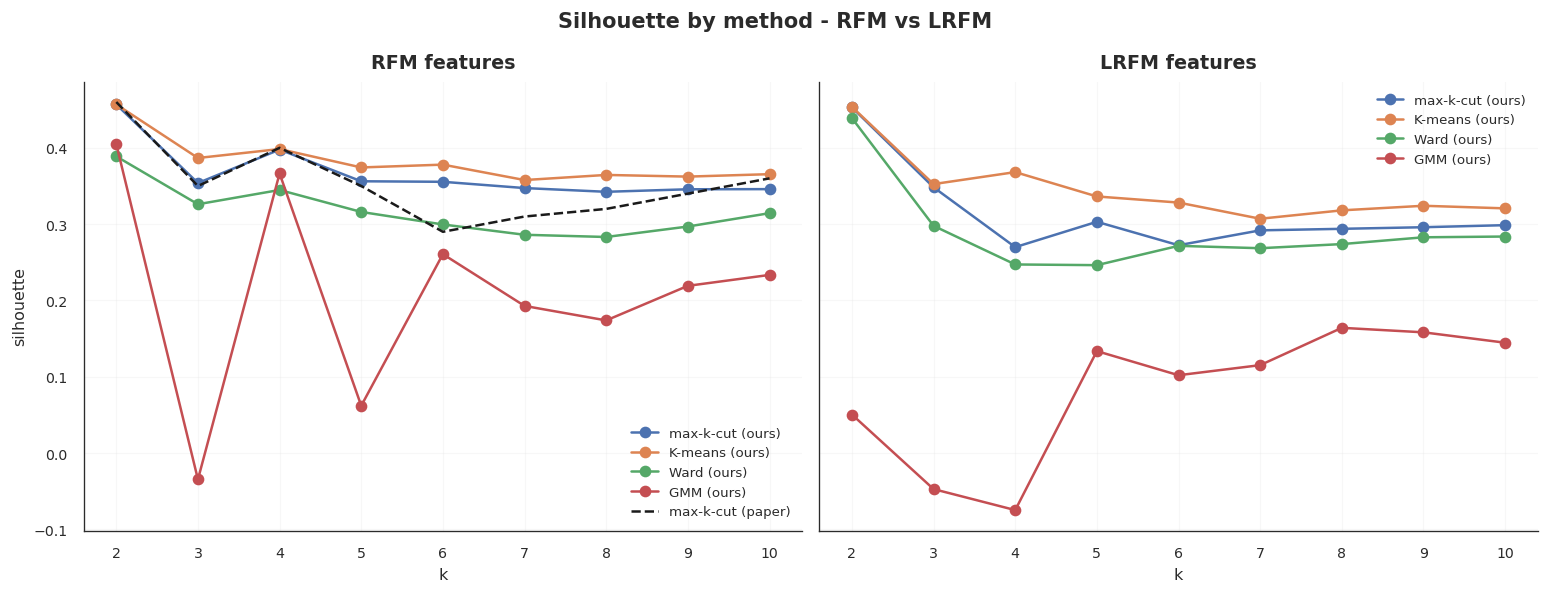
\includegraphics[width=0.95\textwidth]{figures/comparison_silhouette.png}
\caption{Silhouette index by clustering method for RFM (left) and LRFM (right) score features; the dashed line is the baseline's reported max-$k$-cut values \cite{vianna2026}.}\label{fig:compare}
\end{figure}

\subsection{LRFM segmentation and loyalty profiles}\label{subsec:lrfm}
Adding the tenure dimension lowers the silhouette index (e.g.\ $0.27$ versus $0.40$ at $k=4$), as expected when a fourth dimension is added. The value of LRFM is not metric but managerial: at $k=4$ the loyalty-ranked clusters (Table~\ref{tab:loyalty}, Figure~\ref{fig:profile}) separate customers that pure RFM conflates. In particular, among otherwise high-scoring customers, $L$ distinguishes long-tenured loyal customers from recently acquired high-spenders---two groups that warrant different retention and growth strategies. As a concrete instance, of the $470$ customers with the top RFM score $5$-$5$-$5$, the tenure dimension spreads them across $L$-scores $2$ to $5$ with mean tenures of $84$, $248$, $473$ and $698$ days; RFM places all $470$ in a single cell, whereas LRFM separates the newcomers from the long-standing loyalists. The Very-high-loyalty cluster holds about $26\%$ of customers but $78\%$ of revenue, consistent with a strong Pareto effect.

\begin{table}[h]
\caption{LRFM $k=4$ clusters, ranked by Cheng--Chen loyalty distance \eqref{eq:loyalty}.}\label{tab:loyalty}%
\begin{tabular}{@{}lrrrrrr@{}}
\toprule
Cluster (loyalty) & $\bar R$ & $\bar F$ & $\bar M$ & $\bar L$ & \% cust. & \% rev.\\
\midrule
Very high & 4.2 & 4.7 & 4.6 & 4.6 & 26 & 78\\
High      & 3.2 & 3.5 & 3.5 & 3.6 & 25 & 14\\
Medium    & 2.5 & 2.4 & 2.3 & 2.5 & 24 & 5\\
Low       & 1.9 & 1.2 & 1.5 & 1.2 & 25 & 3\\
\botrule
\end{tabular}
\end{table}

\begin{figure}[h]
\centering
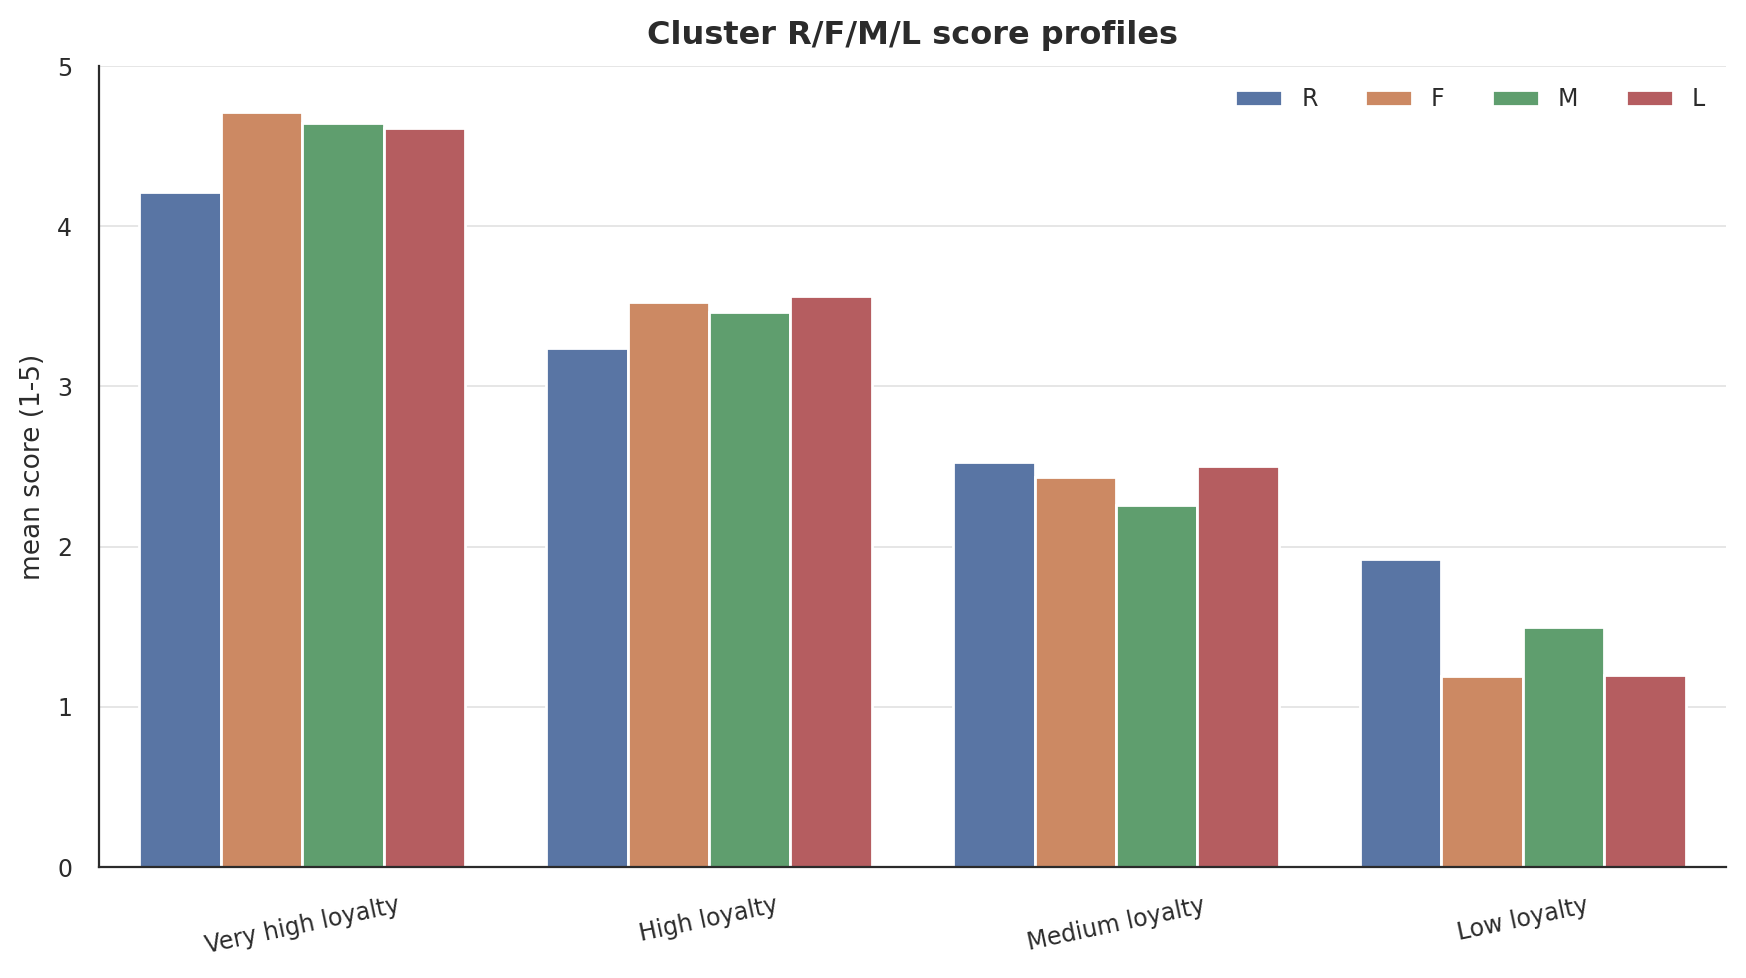
\includegraphics[width=0.85\textwidth]{figures/viz_segment_profile_bars.png}
\caption{Mean R/F/M/L scores per LRFM loyalty cluster.}\label{fig:profile}
\end{figure}

\subsection{Solver validation}\label{subsec:solverval}
On small instances where brute-force enumeration is tractable, the licence-free solver matched the global optimum in $40/40$ randomly generated cases. On the full reduced graphs it solves all $k$ in seconds (RFM $k{=}10$ in $0.15$\,s; LRFM $k{=}10$ in $6.7$\,s) and, with $200$ restarts, returned the best observed cut in every repeated run. Its cut objectives match the baseline's published values to within $0.02\%$, and exceed the baseline's time-limited solver output at the values of $k$ where that solver did not certify optimality.

\section{Discussion}\label{sec:discuss}
Three findings stand out. First, the graph-based baseline reproduces faithfully, and a licence-free heuristic suffices to obtain optimal-quality cuts on the reduced graph, removing a practical barrier to adoption. Second, the LRFM extension does not improve the silhouette index; rather, it trades cluster separation for an actionable tenure dimension. Framing the contribution on managerial value, not on a clustering metric, is therefore essential and honest. Third, when every method is run on identical features, K-means is competitive with max-$k$-cut, suggesting that part of the previously reported gap reflects preprocessing rather than the algorithm itself.

The study has limitations. The dataset contains no campaign-response label, so response-rate or uplift modelling is not possible; we therefore restrict claims to segmentation. The $+1.5\%$ monetary discrepancy reflects an undocumented preprocessing choice in the baseline. Finally, the $L$--$F$ score correlation is $\rho\approx0.85$, comparable to the $F$--$M$ score correlation of $0.81$ already accepted within the RFM model, so $L$ is not disproportionately redundant.

\section{Conclusion}\label{sec:conclusion}
We reproduced a recent graph-based max-$k$-cut RFM segmentation method, extended it to LRFM with a tenure dimension while preserving its vertex-reduction guarantee, and replaced its commercial-solver dependency with a validated, licence-free heuristic. The LRFM segments isolate newly acquired from long-tenured loyal customers---an actionable distinction RFM cannot make---at the cost of a lower silhouette index, and we found K-means to be competitive once features are held constant. Future work includes richer behavioural graphs (e.g.\ co-purchase edges), additional tenure-based variables, and validation on datasets that include marketing-response labels.

\backmatter

\bmhead{Acknowledgements}
The authors thank their supervisor, Hoang Linh Nguyen (FPT University), for guidance throughout this project, carried out for the course DAP391m.

\section*{Declarations}
\begin{itemize}
\item \textbf{Funding.} Not applicable.
\item \textbf{Conflict of interest.} The authors declare no competing interests.
\item \textbf{ORCID.} Cong Minh Nguyen: 0009-0009-6348-0359.
\item \textbf{Data availability.} The Online Retail II dataset is publicly available from the UCI Machine Learning Repository \cite{onlineretail2019}.
\item \textbf{Code availability.} The full pipeline (cleaning, SQL scoring, solver, evaluation, figures) is available from the authors on request.
\item \textbf{Author contributions.} All authors contributed to the study design, implementation and writing, and approved the final manuscript.
\end{itemize}

\bibliography{refs}

\end{document}
